\newlecture

\setcounter{section}{1}
%\def\textbookchapter{Chapter 9: Multivariable and Vector Functions}
\def\coursetopicnumber{I}
\def\textbooksection{9.2} % corresponding textbook section
\def\topic{Vectors} % this is the printed title
\def\shorttopic{Vectors} % short topic
\def\textbookname{Active Calculus} % this is the textbook
\def\textbooksectionurl{https://activecalculus.org/vector/S-9-2-Vectors.html} % URL for textbook section
\def\handoutday{} % this is the printed date

%%%%%%%%% DOCUMENT CONTENT STARTS BELOW

\thispagestyle{plain}
\topstuff
\section{\topic{} \booklink{}}
%\section{\href{\textbooksectionurl}{\topic{}}}
\subsection{Representations of vectors}
\begin{defn}[Vector]
A \emph{vector} (or \emph{displacement vector}) is an arrow that has a tail at one end and a head at the other end.
\end{defn}
\vspace{1in}

Vectors exist in $\mathbb{R}$, $\mathbb{R}^2$, $\mathbb{R}^3$, etc. We'll focus on vectors in $\mathbb{R}^2$ since any drawing surface is essentially $\mathbb{R}^2$. Note that the ideas we'll see apply in any dimension.

Any vector has two important characteristics: 
\begin{itemize}
    \item its \emph{direction} (i.e., \hide{the direction in which it points), and}
    \item its \emph{magnitude} (i.e., \hide{its length).}
\end{itemize}

\begin{framed}
    Two vectors are equal if \hide{they point in the same direction and have the same magnitude.} \\ \mbox{} \\ \mbox{} 
\end{framed}

\vfill

To distinguish vectors from real numbers, we put an arrow over the vector's name (like $\vec{v}$) to indicate that it is a vector.  In most books -- including ours! --  vectors are written in bold (like $\mathbf{v}$).


Any vector $\vec{v}$ can be thought of as an arrow from a point $P$ to a point $Q$. We write $\vec{v}=\vec{PQ}$.

%% The following command gives empty axes.
\newcommand{\AxesForVectors}{
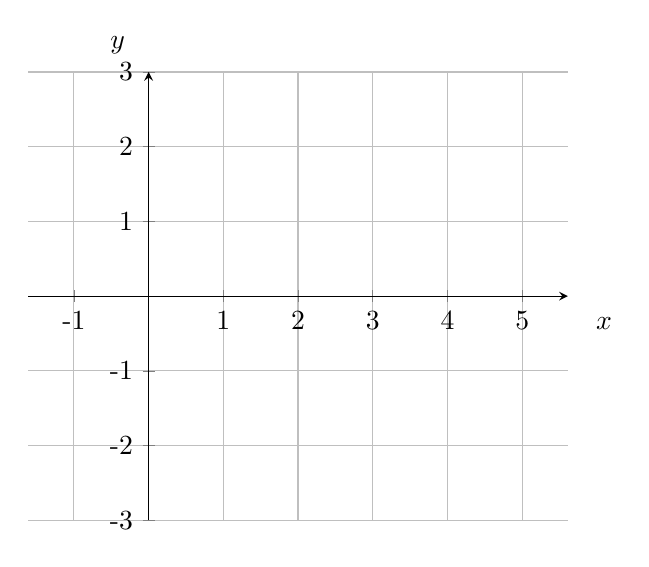
\begin{tikzpicture}
  \begin{axis}[grid=both,ymin=-3,ymax=3,xmax=5,xmin=-1,xtick={-1,0,1,2,3,4,5},ytick={-3,-2,-1,0,1,2,3},xticklabels={-1,0,1,2,3,4,5},yticklabels={-3,-2,-1,0,1,2,3},
               axis lines = middle,axis equal=true,xlabel=$x$,ylabel=$y$,label style =
               {at={(ticklabel cs:1.1)}}]
  \end{axis}
\end{tikzpicture}}

\begin{ex}
    Let $P=(1,2)$ and $Q=(4,0)$. Draw $\vec{v}=\vec{PQ}$. If we shift $\vec{v}$ to start at the point $(0,1)$, where does it end? What if we shifted $\vec{v}$ to start at the origin?
    
    \includegraphics[width=.3\textwidth]{tikz-pictures/section-9.2-pic1-axes-for-vectors.pdf}
\end{ex}

\pagebreak 

Let $O$ denote the origin. Just as in the previous example, any vector can be moved so that it starts at $O$.

\begin{defn}[Standard position, component form, position vector]
\label{defn:position-vector}
    When a vector starts at the origin, we say that it is in \emph{standard position}.
    
    If a vector $\vec{v}$ in standard position ends at a point $P=(a,b)$, we write 
    \[
        \vec{v}=\vec{OP}=\phantom{\langle a,b\rangle,}\hspace{2in}
    \]
    which is the \emph{component form of $\vec{v}$}. This is a \emph{position vector} for the point $P$.
\end{defn}

\vspace{1in}

\begin{ex}
    For $P=(2,-1)$ and $Q=(4,2)$, let $\vec{v}=\vec{PQ}$. Draw $\vec{v}$, then draw $\vec{v}$ as a position vector, and then write $\vec{v}$ in component form.
    
    \includegraphics[width=.3\textwidth]{tikz-pictures/section-9.2-pic1-axes-for-vectors.pdf}
\end{ex}

\begin{framed}
    In general, if $\vec{v}=\vec{PQ}$ with $P=(x_1,y_1)$ and $Q=(x_2,y_2)$, then 
    \medskip 

    $\vec{v}=\phantom{\langle x_2-x_1, y_2-y_1\rangle.}$\\ \mbox{}
\end{framed}
\begin{ex}
    For $P=(4,-1)$ and $Q=(-2,3)$, let $\vec{v}=\vec{PQ}$. Write $\vec{v}$ in component form.
\end{ex}

\vfill

\subsection{Equality of vectors}
\begin{framed} 
    Two position vectors $\vec{u}=\langle u_1,u_2\rangle$ and $\vec{v}=\langle v_1,v_2\rangle$ are equal if and only if \hide{$u_1=v_1$ and $u_2=v_2$.}\\
\end{framed}
Note: These boxed statements extend to vectors in $\mathbb{R}^3$ (and beyond).
\pagebreak 

\subsection{Operations on vectors}
\begin{defn}[Vector addition]
    For vectors $\vec{v}=\langle v_1,v_2\rangle$ and $\vec{w}=\langle w_1,w_2\rangle$ in $\mathbb{R}^2$, we add $\vec{v}$ and $\vec{w}$ as follows:
    \[
        \vec{v}+\vec{w}=\langle v_1,v_2\rangle+\langle w_1,w_2\rangle = \phantom{\langle v_1+w_1,v_2+w_2\rangle.}\hspace{2in}
    \]
\end{defn}
We call this \emph{component-wise addition}. Vector addition in $\mathbb{R}^3$ works the same way.

\begin{ex}
    Let $\vec{v}=\langle 2,-3\rangle$ and $\vec{w}=\langle 5,2\rangle$. Compute $\vec{v}+\vec{w}$.
\end{ex}

\vspace{1in}

\begin{defn}[Scalar]
    A \emph{scalar} is a real number.
\end{defn}
\begin{ex}
    Write down a few examples of scalars.
\end{ex}
%Here are a few examples of scalars: $3/5$, $-\pi$, $142.7$, and $0$.

\vspace{1in}

We can multiply any vector by a scalar.
\begin{defn}[Scalar multiple]
    If $c$ is a scalar and $\vec{v}$ is a vector, then $c\vec{v}$ is a vector. We call $c\vec{v}$ a \emph{scalar multiple} of $\vec{v}$.
\end{defn}

In component form, if $\vec{v}=\langle v_1,v_2\rangle$, then $c\vec{v}=c\langle v_1,v_2\rangle=\phantom{\langle c v_1, cv_2\rangle.}$

\begin{ex}\label{ex:parallel-vectors}
    For $\vec{v}=\langle 2,1\rangle$, compute $c\vec{v}$ for $c=3$, $c=-1$, and $c=0$. Then draw $\vec{v}$ and these vectors on the axes below.
\end{ex}
\mbox{} \hfill \includegraphics[width=.4\textwidth]{tikz-pictures/section-9.2-pic2-axes-for-more-vectors.pdf}

\vfill

\noindent Notation: For any vector $\vec{v}$, $-\vec{v}$ means $(-1)\vec{v}$.
\begin{defn}[Zero vector]
    The \emph{zero vector}, written $\vec{0}$, is the vector whose components are all 0. In $\mathbb{R}^2$, $\vec{0}=\langle 0,0\rangle$. In $\mathbb{R}^3$, $\vec{0}=\langle 0,0,0\rangle$.
\end{defn}

\pagebreak 

Visually, we see that the vectors in Exercise~\ref{ex:parallel-vectors} are parallel to each other. Here's our definition.

\begin{defn}[Parallel vectors]
    Vectors $\vec{u}$ and $\vec{v}$ are \emph{parallel} if \hide{one of them is a scalar multiple of the other.}
\end{defn}

\vspace{.7in}

\begin{ex}
    Consider the vectors $\vec{v}=\langle 1,2\rangle$, $\vec{w}=\langle 3,-4\rangle$, and $\vec{u}=\langle -5,-10\rangle$. Are any of these vectors parallel to each other?
\end{ex}

\vspace{1.5in}

Now that we can add vectors and multiply vectors by scalars, we can subtract vectors.
\begin{defn}[Vector subtraction]
    For vectors $\vec{v}$ and $\vec{w}$, we subtract $\vec{w}$ from $\vec{v}$ as follows:
    \[
        \vec{v}-\vec{w}=\phantom{\vec{v}+(-1)\vec{w}.}\hspace{2in}
    \]
    In particular, if $\vec{v}=\langle v_1,v_2\rangle$ and $\vec{w}=\langle w_1,w_2\rangle$ are vectors in $\mathbb{R}^2$, then
    \[
        \vec{v}-\vec{w}=\langle v_1,v_2\rangle-\langle w_1,w_2\rangle = \phantom{\langle v_1-w_1,v_2-w_2\rangle.}\hspace{2in}
    \]
\end{defn}
%(In other words, $-\vec{w}$ means $(-1)\vec{w}$.)
\bigskip 

\begin{defn}[Standard unit vectors]
    In $\mathbb{R}^2$, we have two special vectors: 
    \[
        \ii =\langle 1,0\rangle \text{ and } \jj =\langle 0,1\rangle.
    \]
    In $\mathbb{R}^3$, we have three special vectors:
    \[
        \ii =\langle 1,0,0\rangle \text{ and } \jj =\langle 0,1,0\rangle \text{ and } \kk =\langle 0,0,1\rangle.
    \]
    These are all \emph{standard unit vectors}.
\end{defn}

\begin{ex}
    Draw $\ii $ and $\jj $ in $\mathbb{R}^2$. Draw $\ii $, $\jj $, and $\kk $ in $\mathbb{R}^3$.
\end{ex}

\vspace{1.5in}

\begin{ex}
    Let $\vec{v}=3\ii +4\jj +6\kk $. Write $\vec{v}$ in component form.
\end{ex}

\vspace{1in}

\pagebreak 
In terms of the standard unit vectors, 
\begin{multicols}{2}
    \begin{itemize}
        \item $\langle a,b\rangle = \phantom{a\ii +b\jj }$
        \item $\langle a,b,c\rangle = \phantom{a\ii +b\jj +c\kk .}$
    \end{itemize}
\end{multicols}
\bigskip 

We have two equivalent notations for vectors: component form with the angle brackets; and in terms of standard unit vectors. Both notations are useful.

\subsection{Properties of vector operations}
We now know how to add vectors together and how to multiply them by scalars. In general, a set of vectors like this forms a \emph{vector space}. (For a course on vector spaces, take Linear Algebra!)

In a vector space, the following properties which hold for any vectors $\vec{u}, \vec{v}, \vec{w}$ and any scalars $a$ and $c$:
\begin{enumerate}[label=\arabic*.]
    \item $\vec{u}+\vec{v}=\phantom{\vec{v}+\vec{u}}$ \hfill (Commutative property of addition)
    \item $(\vec{u}+\vec{v})+\vec{w}=\phantom{\vec{u}+(\vec{v}+\vec{w})}$ \hfill (Associative property of addition)
    \item $\vec{v}+\vec{0}=\phantom{\vec{v}}$ \hfill (Additive identity)
    \item $\vec{v}+(-\vec{v})=\phantom{\vec{0}}$ \hfill (Additive inverse)
    \item $c(\vec{u}+\vec{v})=\phantom{c\vec{u}+c\vec{v}}$ \hfill (Distributive property 1)
    \item $(a+c)\vec{v}=\phantom{a\vec{v}+c\vec{v}}$ \hfill (Distributive property 2)
    \item $0\vec{v}=\phantom{\vec{0}}$ \hfill (Multiplication by zero scalar)
    \item $c\vec{0}=\phantom{\vec{0}}$ \hfill (Multiplication of zero vector)
    \item $1\vec{v}=\phantom{\vec{v}}$ \hfill (Multiplicative identity)
    \item $a(c\vec{v})=\phantom{(ac)\vec{v}}$ \hfill (Associative property of scalar multiplication)
\end{enumerate}
Each property is relatively straightforward to show if you write each vector in component form.
\bigskip 

\begin{ex}
    Let $\vec{v}=2\ii -3\jj $ and $\vec{w}=5\ii +2\jj $.
    Suppose 
    \[
        2\vec{v}+3\vec{x}=\vec{w}+\jj .
    \]
    Solve for $\vec{x}$.
\end{ex}

\pagebreak 

\subsection{Geometric interpretation of vector operations}
We know how to visualize scalar multiplication. There are nice geometric interpretations for vector addition and subtraction, too.

For vector addition, we use the ``head-to-tail'' method. If we want to compute $\vec{v}+\vec{w}$, we select a starting point $P$, draw $\vec{v}$ as starting at $P$ and ending at some point $Q$, and then draw $\vec{w}$ as starting at $Q$ and ending at some point $R$. 

\vspace{2in}

In other words, if $\vec{v}=\vec{PQ}$ and $\vec{w}=\vec{QR}$, then $\vec{v}+\vec{w}=\vec{PR}$. This means that $\vec{v}$, $\vec{w}$, and $\vec{v}+\vec{w}$ form three sides of a triangle.

For the picture above, we connected the head of $\vec{v}$ to the tail of $\vec{w}$. Since $\vec{v}+\vec{w}=\vec{w}+\vec{v}$, we could draw the vectors in the opposite order. This gives rise to the ``parallelogram rule'' for adding vectors.

\vspace{2in}

For vector subtraction, we have two approaches. First, to compute $\vec{v}-\vec{w}$, we know that
\[
    \vec{v}-\vec{w}=\vec{v}+(-\vec{w}).
\]
So, if we can draw $\vec{v}$ and $-\vec{w}$, then we can add them with the method above.

Alternatively, we can draw the vectors $\vec{v}$ and $\vec{w}$ both starting from the same point. Then, draw the vector from the head of $\vec{w}$ to the head of $\vec{v}$. That vector is $\vec{v}-\vec{w}$.

\vspace{2in}

\pagebreak 

\subsection{The magnitude of a vector}
\begin{defn}[Magnitude]
    The \emph{magnitude} of a vector $\vec{v}$, denoted $|\vec{v}|$, is the length of $\vec{v}$. (Note: Some other books write this as $||\vec{v}||$.)
\end{defn}

\begin{ex}
    Draw the vector $\vec{v}=\langle 3,-4\rangle$. Compute $|\vec{v}|$.
\end{ex}

\vspace{1.5in}

\begin{framed}
    In general, if $\vec{v}=\langle v_1,v_2\rangle$ is a vector in $\mathbb{R}^2$, then $|\vec{v}|$ is the distance from the origin $(0,0)$ to the point $(v_1,v_2)$. Thus,
    \[
        |\vec{v}|=\phantom{\sqrt{v_1^2+v_2^2}.}\hspace{2in}
    \]
\end{framed}

\begin{framed} 
    More generally, if $\vec{v}=\langle v_1,v_2,\dots,v_n\rangle$ is a vector in $\mathbb{R}^n$, then 
    \[
        |\vec{v}|=\phantom{\sqrt{v_1^2+v_2^2+\dots+v_n^2}.}\hspace{2in}
    \]
\end{framed}

Two notes:
\begin{multicols}{2}
\begin{itemize}
    \item For any scalar $c$, $|c\vec{v}|=|c|\,|\vec{v}|$.
    \item In general, $|\vec{v}+\vec{w}|\ne |\vec{v}|+|\vec{w}|$.
\end{itemize}
\end{multicols}
\bigskip 

\begin{defn}[Unit vector]
    A \emph{unit vector} is a vector $\vec{v}$ with $|\vec{v}|=1$.
\end{defn}
Unit vectors have magnitude 1. Some examples are $\ii$, $\jj$, and $\kk$. And there are many more.

\begin{ex}
    Which of the following are unit vectors?
    \begin{enumerate}
        \item $\vec{v}=\left\langle 1/2,\sqrt{3}/2\right\rangle$
        \item $\vec{w}=\left\langle1,-1,1\right\rangle$
        \item $\vec{u}=\left\langle1/2,1/2,1/2,1/2\right\rangle$
    \end{enumerate}
\end{ex}
\pagebreak 

\begin{ex}
If $\vec{v}$ is any vector other than the zero vector, let $c=1/|\vec{v}|$ and compute $|c\vec{v}|$.
\end{ex}

\vspace{.8in}

\begin{framed}
    \noindent When $\vec{v}\ne \vec{0}$, we can easily find a unit vector $\vec{u}$ that points in the same direction of $\vec{v}$: 
    \[
        \hspace{-3in}\vec{u}=\phantom{\frac{1}{|\vec{v}|}\vec{v}.}
    \]
\end{framed}

\noindent Lingo: When we scale a vector $\vec{v}$ to get a unit vector $\vec{u}$, we have \emph{normalized} $\vec{v}$.

\vfill 

\begin{ex}
    Let $\vec{v}=5\ii -12\jj $.
    \begin{enumerate}
        \item Find a unit vector $\vec{u}$ in the direction of $\vec{v}$.
        \vspace{1.3in}
        \item Find a vector $\vec{w}$ of length 4 in the direction opposite from $\vec{v}$. Write $\vec{w}$ in terms of the standard unit vectors.
        \vspace{1.3in}
    \end{enumerate}
\end{ex}

A \emph{unit circle} is a circle of radius 1. When centered at $(0,0)$, its equation is $x^2+y^2=1$. Starting from the point $(1,0)$, if you travel CCW a distance $\theta$, you get to the point $P=(\cos\theta,\sin\theta)$.

Note that $\theta$ is the angle (in radians) measured above the positive $x$-axis.

\includegraphics[width=.35\textwidth]{tikz-pictures/section-9.2-pic3-unit-circle.pdf}

\pagebreak 

Here's a useful observation. If $\vec{u}$ is a unit vector in standard position in $\mathbb{R}^2$ (meaning its tail is at the origin), then the head of $\vec{u}$ is on the unit circle. Since every point on the unit circle is of the form $(\cos\theta,\sin\theta)$ for some real number $\theta$, every unit vector $\vec{u}$ in $\mathbb{R}^2$ is of the form
\[
    \vec{u}=\phantom{\langle \cos\theta,\sin\theta\rangle}
\]
for some real number $\theta$.

More generally, if $\vec{v}$ is a vector in $\mathbb{R}^2$ that starts at the origin and has magnitude $r$ for some positive number $r$, then the head of $\vec{v}$ is on the circle of radius $r$ centered at the origin.

\begin{ex}
    Let $r>0$ be a scalar. Let $\vec{v}$ be the vector of length $r$ from the origin at an angle $\theta$ above the positive $x$-axis. Write $\vec{v}$ in terms of the standard unit vectors.
\end{ex}

\vspace{3in}

\begin{ex}
    Find a vector $\vec{v}$ of length 5 that points at an angle of $60^\circ$ above the positive $x$-axis.
\end{ex}

\vfill
